\documentclass[xcolor=x11names,compress]{beamer}

%% General document %%%%%%%%%%%%%%%%%%%%%%%%%%%%%%%%%%
\usepackage{graphicx}
\usepackage{tikz}
\usepackage{Tabbing}
\usetikzlibrary{decorations.fractals}
\usepackage{fancyvrb}
%%%%%%%%%%%%%%%%%%%%%%%%%%%%%%%%%%%%%%%%%%%%%%%%%%%%%%

%% Beamer Layout %%%%%%%%%%%%%%%%%%%%%%%%%%%%%%%%%%
\useoutertheme[subsection=false,shadow]{miniframes}
\useinnertheme{default}
\usefonttheme{serif}
\usepackage{palatino}
\usepackage{tabu}
% Links
\usepackage{hyperref}
\definecolor{links}{HTML}{003262}
\hypersetup{colorlinks,linkcolor=,urlcolor=links}

% addition of color
\usepackage{xcolor}
\definecolor{CoolBlack}{rgb}{0.0, 0.18, 0.39}
\definecolor{byellow}{rgb}{0.55037, 0.38821, 0.06142}
\definecolor{dgreen}{rgb}{0.,0.6,0.}
\definecolor{RawSienna}{cmyk}{0,0.72,1,0.45}
\definecolor{forestgreen(web)}{rgb}{0.13, 0.55, 0.13}
\definecolor{cardinal}{rgb}{0.77, 0.12, 0.23}

\setbeamerfont{title like}{shape=\scshape}
\setbeamerfont{frametitle}{shape=\scshape}

\setbeamercolor*{lower separation line head}{bg=CoolBlack} 
\setbeamercolor*{normal text}{fg=black,bg=white} 
\setbeamercolor*{alerted text}{fg=red} 
\setbeamercolor*{example text}{fg=black} 
\setbeamercolor*{structure}{fg=black} 
 
\setbeamercolor*{palette tertiary}{fg=black,bg=black!10} 
\setbeamercolor*{palette quaternary}{fg=black,bg=black!10} 

% Margins
\usepackage{changepage}

\mode<presentation>
{
  \definecolor{berkeleyblue}{HTML}{003262}
  \definecolor{berkeleygold}{HTML}{FDB515}
  \usetheme{Boadilla}      % or try Darmstadt, Madrid, Warsaw, Boadilla...
  %\usecolortheme{dove} % or try albatross, beaver, crane, ...
  \setbeamercolor{structure}{fg=berkeleyblue,bg=berkeleygold}
  \setbeamercolor{palette primary}{bg=berkeleyblue,fg=white} % changed this
  \setbeamercolor{palette secondary}{fg=berkeleyblue,bg=berkeleygold} % changed this
  \setbeamercolor{palette tertiary}{bg=berkeleyblue,fg=white} % changed this
  \usefonttheme{structurebold}  % or try serif, structurebold, ...
  \useinnertheme{circles}
  \setbeamertemplate{navigation symbols}{}
  \setbeamertemplate{caption}[numbered]
  \usebackgroundtemplate{}
}

% Columns
\renewcommand{\(}{\begin{columns}}
\renewcommand{\)}{\end{columns}}
\newcommand{\<}[1]{\begin{column}{#1}}
\renewcommand{\>}{\end{column}}

% adding slide numbers
\addtobeamertemplate{navigation symbols}{}{%
    \usebeamerfont{footline}%
    \usebeamercolor[fg]{footline}%
    \hspace{1em}%
    \insertframenumber/\inserttotalframenumber
}

% equation stuff
\newcommand{\Macro}{\ensuremath{\Sigma}}
\newcommand{\Sn}{\ensuremath{S_N} }
\newcommand{\vOmega}{\ensuremath{\hat{\Omega}}}
\usepackage{mathrsfs}
\usepackage[mathcal]{euscript}
\usepackage{amssymb}
\usepackage{amsthm}
\usepackage{epsfig}
\usepackage{amsmath}
\newcommand{\ve}[1]{\ensuremath{\mathbf{#1}}}
\newcommand{\micro}{\ensuremath{\sigma}}
\newcommand{\detR}{\ensuremath{\Sigma}}

% title stuff for footer
\title{The PyNE Software Library}
\author{R.\ N.\ Slaybaugh}
\date{22 October 2014}

%%%%%%%%%%%%%%%%%%%%%%%%%%%%%%%%%%%%%%%%%%%%%%%%%%%%%%
\begin{document}



%%%%%%%%%%%%%%%%%%%%%%%%%%%%%%%%%%%%%%%%%%%%%%%%%%%%%%
%%%%%%%%%%%%%%%%%%%%%%%%%%%%%%%%%%%%%%%%%%%%%%%%%%%%%%
\begin{frame}
\title{The PyNE Software Library: Why and How?}
%\subtitle{}
\author{
        \includegraphics[height=2cm]{../bk}\\R.\ N.\ Slaybaugh \\ Univ.\ of Cal.\ Berkeley}

\date{ANS Nor Cal Meeting \\ 22 October 2014\\ Alfred's Stakehouse, San Francisco, CA}
\titlepage
\end{frame}

%------------------------------------------------------
\begin{frame}{Outline}

	\begin{columns}
  	\begin{column}{0.4\textwidth}
	    \begin{itemize}
        \item PyNE \cite{pyne}: what is it?
        \item Demo
        \item Current initiatives
        \item PyNE as a research tool
        \item Get involved!
	    \end{itemize}
  	\end{column}
 	%
 	\begin{column}{0.5\textwidth}
 	   \begin{center}
 	   \begin{figure}
       
\includegraphics[height=3.5cm]{pyne-icon-big}
	   \end{figure}
 	   \end{center}
  	\end{column}
	\end{columns}

\end{frame}

%%%%%%%%%%%%%%%%%%%%%%%%%%%%%%%%%%%%%%%%%%%%%%%%%%%%%%
%%%%%%%%%%%%%%%%%%%%%%%%%%%%%%%%%%%%%%%%%%%%%%%%%%%%%%
\section{PyNE \cite{pyne}: what is it?}
\begin{frame}{What is PyNE?}

    PyNE is \textit{the} open source nuclear engineering toolkit.
    \vspace*{1em}
    \begin{itemize}
    \item PyNE is a \textit{library of composable tools} used to build 
    nuclear science and engineering applications
    \item It is \textit{permissively licensed} (2-clause BSD)
    \item It supports both a \textit{C++} and a \textit{Python} API
    \item The name 'PyNE' is a bit of a misnomer since most of the code 
    base is in C++ but most daily usage happens in Python
    \item \textit{v0.4} is the current, stable release
    \item As an organization, PyNE was born in April 2011 
    (however, core parts of PyNE have existed since 2007)
    \end{itemize}

\end{frame}

%------------------------------------------------------
\begin{frame}{What are the Goals of PyNE?}

    \begin{columns}
    \begin{column}{0.4\textwidth}
        To help nuclear engineers:
        \begin{itemize}
        \item be more \textit{productive} (don't reinvent the wheel!)
        \item have the best \textit{solvers}
        \item have a clear and useful \textit{API}
        \item write really great code
        \item \textit{teach} the next generation
        \end{itemize}
  	\end{column}
   	%
 	\begin{column}{0.5\textwidth}
 	   \begin{center}
 	   \begin{figure}
 	   \includegraphics[height=1.25in,clip]{data_sources_thumb}  \\
       \includegraphics[height=1.25in,clip]{half_life_thumb}
	   \end{figure}
 	   \end{center}
  	\end{column}
	\end{columns}

\end{frame}

%Python for Nuclear Engineering, or PyNE (http://pyne.io/), is a collaborative, open source project consisting of a collection of
%computational tools pertinent to nuclear engineering analysis and simulations.
%PyNE primarily provides a common Python interface for code written in C++,
%Python, and Fortran. This allows fundamental components of PyNE to easily be
%combined to form powerful and complex programs. These fundamental components
%include canonical nuclide and reaction naming conventions, material handling,
%nuclear data and cross-section reading, mesh operations, and
%physics-code-specific input and output parsing.
%
%This presentation will begin with a discussion about the background and philosophy behind PyNE and include a demonstration of how PyNE could be used in a project. I will also cover some of the current developments, with a focus of how I'm using PyNE as a tool for my research in computational methods for neutral particle transport. 
%%%%%%%%%%%%%%%%%%%%%%%%%%%%%%%%%%%%%%%%%%%%%%%%%%%%%%
%%%%%%%%%%%%%%%%%%%%%%%%%%%%%%%%%%%%%%%%%%%%%%%%%%%%%%
\section{Demo}
\begin{frame}{What Can PyNE Do?}

    \begin{itemize}
    \item Nuclear data and cross-section reading/processing
    \item Material handling
    \item Canonical nuclide and reaction naming conventions
    \item Mesh operations
    \item MCNP and Serpent input/output parsing
    \item Fuel cycle functionality (transmutation, enrichment)
    \item There's more, and the list continues to grow
    \end{itemize}
    
    The idea is to be able to easily combine components and avoid redeveloping
    utilities someone else has developed.
    
    \begin{center}
    \textbf{Demos}: (1) Data sources \hspace*{3 em} (2) Enrichment
    \end{center}

\end{frame}

%%%%%%%%%%%%%%%%%%%%%%%%%%%%%%%%%%%%%%%%%%%%%%%%%%%%%%
%%%%%%%%%%%%%%%%%%%%%%%%%%%%%%%%%%%%%%%%%%%%%%%%%%%%%%
\section{Current initiatives}
\begin{frame}{What are we Working on Now?}

    The biggest push: V\&V $\rightarrow$ methodically making PyNE compliant 
    with the QA standards we've ratified, based on the ASME NQA-1 standards
    \cite{pyne_vnv}

    \vspace*{1 em}
    Many other items (large and small) in our "ticket" list
    
    \begin{center}
 	\begin{figure}
 	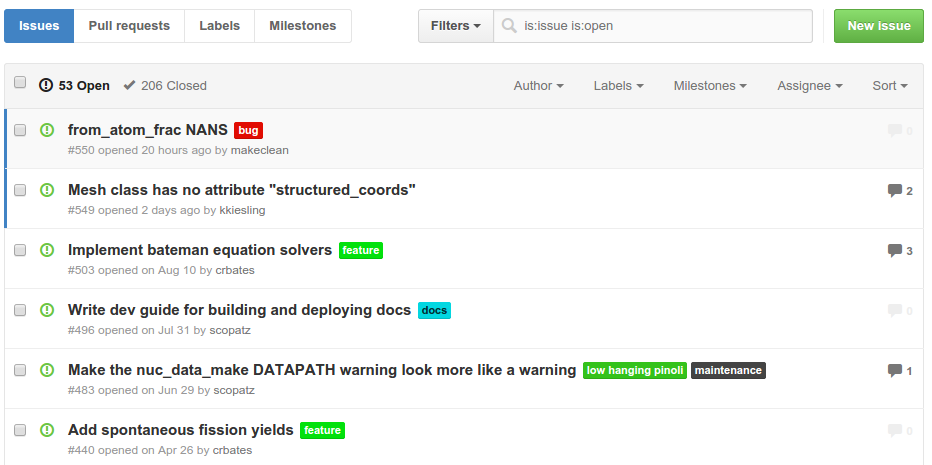
\includegraphics[height=1.75in,clip]{PyNE-tickets}
    \end{figure}
 	\end{center}
    
\end{frame}

%------------------------------------------------------
\begin{frame}{Verification and Validation}

    \textbf{Verification}: Have we built the software correctly?\\
    \textbf{Validation}: Have we built the right software?
    
    \vspace*{1 em}
    Strategies employed by PyNE:
    \begin{itemize}
    \item Version control
    \item Formal review process
    \item Documentation: theory manual, user's guide, developer's guide, API
    \item Test suite
    \item Continuous Integration
    \end{itemize}

\end{frame}

%%%%%%%%%%%%%%%%%%%%%%%%%%%%%%%%%%%%%%%%%%%%%%%%%%%%%%
%%%%%%%%%%%%%%%%%%%%%%%%%%%%%%%%%%%%%%%%%%%%%%%%%%%%%%
\section{PyNE as a research tool}  
\begin{frame}{PyNE as a research tool}

    \textbf{Insight}: PyNE lets us access the physics, have real materials, 
    add mesh, and handle many details easily...
    
    \vspace{1 em}
    \textbf{Idea}: perfect environment for investigating numerical methods that 
    are impacted by materials, mesh, etc. 
    
    \vspace{1 em}
    \textbf{My Plan:} Plug-And-Play Solver Research Environment

 	\begin{figure}
    
\includegraphics[height=3cm]{pyne-icon-big}
	\end{figure}
    
\end{frame}

%------------------------------------------------------
\begin{frame}{What Are We Sovling?}

    I study how to solve the Boltzmann neutral particle transport equation
    more efficiently:
    %   
    \begin{align}
    [\vOmega \cdot \nabla + \Macro(\vec{r}, E)] &\psi(\vec{r}, \vOmega, E)  = 
     \chi(E)   \int_0^{\infty} dE' \:\nu \Macro_{f}(\vec{r}, E') \int_{4\pi} d\vOmega'
     \:\psi(\vec{r}, \vOmega', E')  \nonumber \\
     &+ \int_0^{\infty} dE' \int_{4\pi} d\vOmega' \:\Macro_{s}(\vec{r}, E' \to E,
     \vOmega' \cdot \vOmega) \psi(\vec{r}, \vOmega', E')  \nonumber
    \end{align}

    Converted to operator form:
    \begin{align}
    \mathbf{L} \psi &= \mathbf{MS}\phi + \frac{1}{k}\mathbf{MF}\phi \nonumber\\
    \phi &= \mathbf{D}\psi \nonumber
    \end{align}

\end{frame}

%------------------------------------------------------
\begin{frame}{How Do We Discretize It?}

    \begin{columns}
    \begin{column}{0.5\textwidth}
        \begin{center}
 	    \begin{figure}
 	    \includegraphics[height=1.75in,clip]{../figs/spatial-discretiztation2}
        \end{figure}
 	    \end{center}
  	\end{column}
   	%
 	\begin{column}{0.4\textwidth}
        There are many many ways to \textbf{\textcolor{dgreen}{discretize}} this problem
        \begin{itemize}
        \item Spatial discretization methods
        \item Angular quadratures
        \item Energy group structures
        \end{itemize}
    
        \vspace*{1 em}
        Each \textbf{\textcolor{dgreen}{discretization}} scheme results in different 
        numerical properites and/or solution strategies
  	\end{column}
	\end{columns}
 
\end{frame}

%------------------------------------------------------
\begin{frame}{How Do We Solve It?}

    \begin{columns}
    \begin{column}{0.4\textwidth}
        There are many many ways to \textbf{\textcolor{dgreen}{solve}} this problem
        \begin{itemize}
        \item Inner iteration methods
        \item Outer iteration methods
       \item Eigenvalue iteration methods
        \item Preconditioners
        \end{itemize}
    
        Each \textbf{\textcolor{dgreen}{solution}} method results in different
       numerical properites and/or solution strategeies
  	\end{column}
   	%
 	\begin{column}{0.5\textwidth}
 	   \begin{center}
 	   \begin{figure}
 	   \includegraphics[height=2.5in,clip]{solverLayers}
       \end{figure}
 	   \end{center}
  	\end{column}
	\end{columns}
	
\end{frame}
% All of the discretization choices and all of the solution stratgies create a complex set of choices

%------------------------------------------------------
\begin{frame}{Oh, and Physics}

    The physics of any specific problem also has a large impact on the
    problem's properties
    
    \begin{columns}
    \begin{column}{0.45\textwidth}
 	   \begin{center}
 	   \begin{figure}
 	   \includegraphics[height=1.75in,clip]{../figs/Fe-D2O-C}
 	   \caption{Iron-D2O-Graphite block energy S matrix; Evans et al.}
       \end{figure}
 	   \end{center}
  	\end{column}
   	%
 	\begin{column}{0.45\textwidth}
 	   \begin{center}
 	   \begin{figure}
 	   \includegraphics[height=1.75in,clip]{../figs/Fe-D2O-C-space-energy}
 	   \caption{Iron-D2O-Graphite energy-space-angle S matrix; Evans et al.}
       \end{figure}
 	   \end{center}
  	\end{column}
	\end{columns}
       
\end{frame}

%------------------------------------------------------
\begin{frame}{Plug-And-Play Research Environment}

    \textbf{Insight}: PyNE lets us access the physics, have real materials, 
    and handle many details easily...
    
    \vspace{1 em}
    \textbf{Idea}: perfect for an investigation environment
    
    \begin{itemize}
    \item Easy to add solver components for each part of phase space
    \item Can plug into properties that facilitate real problem investigation
    \item Flexible environment
    \item Start with standard methods
    \item Provide API for adding new/alternative methods
    \end{itemize}
    
\end{frame}

%%%%%%%%%%%%%%%%%%%%%%%%%%%%%%%%%%%%%%%%%%%%%%%%%%%%%%
%%%%%%%%%%%%%%%%%%%%%%%%%%%%%%%%%%%%%%%%%%%%%%%%%%%%%%
\section{Get involved!}
\begin{frame}{Why Would I Get Involved?}

As a \underline{\textcolor{byellow}{\textbf{user}}} you could do your work or research with PyNE.  Even if you have your own software that looks and behaves similarly to some aspects of PyNE, using PyNE will mean that you no longer have to develop AND maintain that functionality.

\vspace*{2 em}
As a \underline{\textcolor{byellow}{\textbf{developer}}} you should be selfish.  Contribute to PyNE in ways that support the work that you are doing. If a feature you want is not in PyNE right now, chances are that other people want to see that feature too! This will help your future self as much as future other people.

\end{frame}

%------------------------------------------------------
\begin{frame}{How Can I Get Involved?}

    \textcolor{byellow}{Contact PyNE}
    \begin{itemize}
    \item Website: \href{http://pyne.io/}{http://pyne.io/}
    \item User's Mailing List: \href{pyne-users@googlegroups.com}{pyne-users@googlegroups.com}
    \item Developer's List: \href{pyne-dev@googlegroups.com}{pyne-dev@googlegroups.com}
    \item GitHub: \href{https://github.com/pyne/pyne}{https://github.com/pyne/pyne}
    \end{itemize}
    
    \vspace*{2 em}
    \textcolor{byellow}{What goes into PyNE?}

    Anything that is not export controllable, proprietary, 
    or under HIPPA restrictions!  (If you have questions, ask)
  
\end{frame}


%%%%%%%%%%%%%%%%%%%%%%%%%%%%%%%%%%%%%%%%%%%%%%%%%%%%%%
%%%%%%%%%%%%%%%%%%%%%%%%%%%%%%%%%%%%%%%%%%%%%%%%%%%%%%
\section*{}
\begin{frame}[fragile]{Questions?}

    \begin{center}
    \includegraphics[height=3in,clip]{../questions-comic}  
    \end{center}
  
\end{frame}

% --------------------------------------------------------------
\begin{frame}[fragile]{PyNE In the Literature}

    \begin{itemize}
    \item Intro: "PyNE: Python For Nuclear Engineering" \cite{pyne_intro}
    \item Progress reports: \cite{scopatz_pyne}, \cite{pyne_progress}
    \item In research: \cite{Biondo2014}, \cite{MarquezDamian2014280}, \cite{Scopatz2013a}
    \item V\&V: "Quality Assurance within the PyNE Open Source \\Toolkit" \cite{pyne_vnv}
    \item Poster at SciPy: \cite{scipy}
    \end{itemize}
  
\end{frame}
% --------------------------------------------------------------
\begin{frame}[allowframebreaks]{References}
	\bibliographystyle{unsrt}
	\bibliography{2014-10-norcal-ans-pyne.bib}
\end{frame}

\end{document}
